\chapter{PDM之碎裂模拟}
\section{碎裂模型}
在近场动力学中,物质的损伤可以直接通过去除粒子之间的 bond 来进行模拟。并且由于近场动力学使用的是积分形式的表述,其在处理不连续问题上也将变得尤为方便。对于弹性或脆性材料,经常使用临界伸长比(critical stretch)来作为碎裂是否发生的标准。\mycite{Silling}{2005}也已经证明, critical stretch 符合损伤力学中的能力释放速率模型,因此是具有物理可信度的。在图形学领域,Levine et al. 的工作\mycite{Levine}{2014}同样使用了一模型,不过其仅仅针对的是脆性材料的碎裂模拟。

在本文工作中,由于不仅仅是考虑弹性行为,还将塑性行为也集成进入本构模型之中。但通常而言,碎裂是否发生又仅仅和弹性行为相关。因此在求解关于弹性的 critical stretch 时,需要将塑性形变排除在外,即

\begin{equation}
s_{ij}^e =\frac{e_{ij}-e_{ij}^p}{|\mathbf{x}_i-\mathbf{x}_j|}.
\end{equation}

然而在实际实验中,本文发现直接使用这一模型将会导致明显的 artifacts(不自然现象)。具体原因是,在这一模型下,离中心粒子越近的邻域粒子在特定情形反而更容易发生碎裂。为缓解这一问题,本文再一次将权重函数 $\omega_{ij}$ 以除法形式引入到碎裂模型中,从而提高具有更小静止长度(rest length)的 bond 的碎裂难度。此外,本文还在实验中还发现对于具有极大刚性系数的脆性材料,在碎裂仿真过程中容易产生过多的小碎块,视觉上反而显得不自然。针对此问题,本文提出的解决方案是随着仿真的进行,以及碎裂程度的不断提高,持续提高再次发生碎裂的阈值。综合上述两点,本文工作最终采用的碎裂模型是:

\begin{equation}
s_{ij}^\omega = (1 + \alpha\phi)\frac{s_{ij}^e}{\omega_{ij}} = (1 + \alpha\phi)\frac{e_{ij}-e_{ij}^p}{\delta},
\end{equation}

其中 $\phi = 1 - \frac{n_i}{N_i}$ 衡量的是粒子 $i$ 和其邻域 $H_\mathbf{x}$ 之间的断裂程度,$N_i$ 是邻域内的初始粒子总数,而 $n_i$ 则是当前还和粒子 $i$ 存在力相互作用的粒子数。不难看出,随着碎裂的进行,$n_i$ 将不断减小。$\alpha$ 参数即用来控制碎小块的数量,其值默认为 0。但可以通过设置非 0 值来加大碎裂进一步发生的难度,从而减少碎小块的数量。图\ref{demo_shatter_control}所示为不同 $\alpha$ 值所产生的不同效果,可以看到随着 $\alpha$ 值的增大,碎小块数量则越来越少。

相对于传统 FEM 的碎裂仿真,基于近场动力学的仿真方法仅仅需要判断碎裂是否发生,而不需要再判断裂纹的生长方向,因此在处理上也更为方便。此外,在 FEM 中往往在碎裂之后需要对拓扑网格进行进一步处理,在剖分之后需要进行 remeshing 操作保证仿真的稳定性。而近场动力学受益于其积分表述,在碎裂发生之后,并不会对后续仿真的稳定性造成影响。

\begin{figure}[!htb]
  \centering
  \captionsetup{justification=centering}
  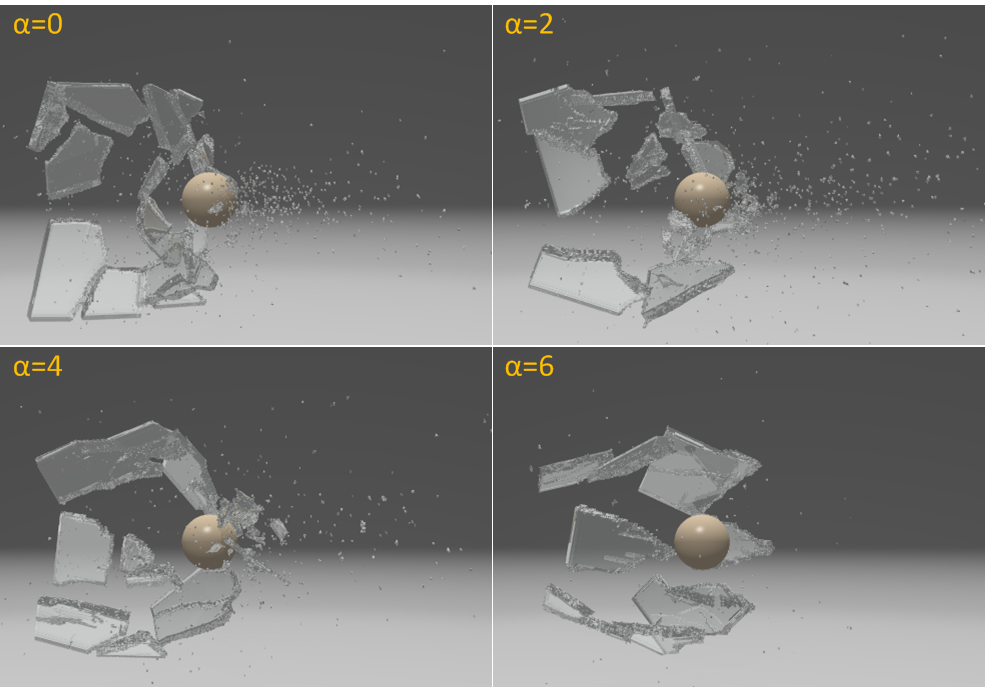
\includegraphics[width=0.6\linewidth]{chap/image/demo_shatter_control}

  \caption{\label{demo_shatter_control}
           不同 $\alpha$ 值的玻璃撞击实验。
          }
\end{figure}

\section{各向异性碎裂}
到目前为止,本文所考虑的形变和碎裂都是各向同性的,亦即材质在各个方向的动力学属性保持一致。本章节则将对本构模型进行进一步拓展,以支持各向异性的碎裂行为。具体而言,本文是通过操作粒子之间的权重函数 $\omega_{ij}$来完成的,而关键思想在于引进各向异性矩阵 $\mathbf{G}$,然后将矩阵 $\mathbf{G}$ 作用于粒子之间的 bond,从而使其在各个方向拥有不同的权重值,来简单地模拟各向异性。对于各向异性材料,权重函数 $\omega_{ij}$ 可具体写为

\begin{equation}
\omega_{ij}=\frac{\delta}{|\mathbf{G}(\mathbf{x}_j-\mathbf{x}_i)|}
\end{equation}

其中各向异性矩阵$\mathbf{G}$其行列式一般为 0,即 $|\mathbf{G}| = 1$。利用这一模型,可以产生非常明显的各向异性碎裂现象。如图\ref{demo_impact_color_map} 所示。

\begin{figure}[!htb]
  \centering
  \captionsetup{justification=centering}
  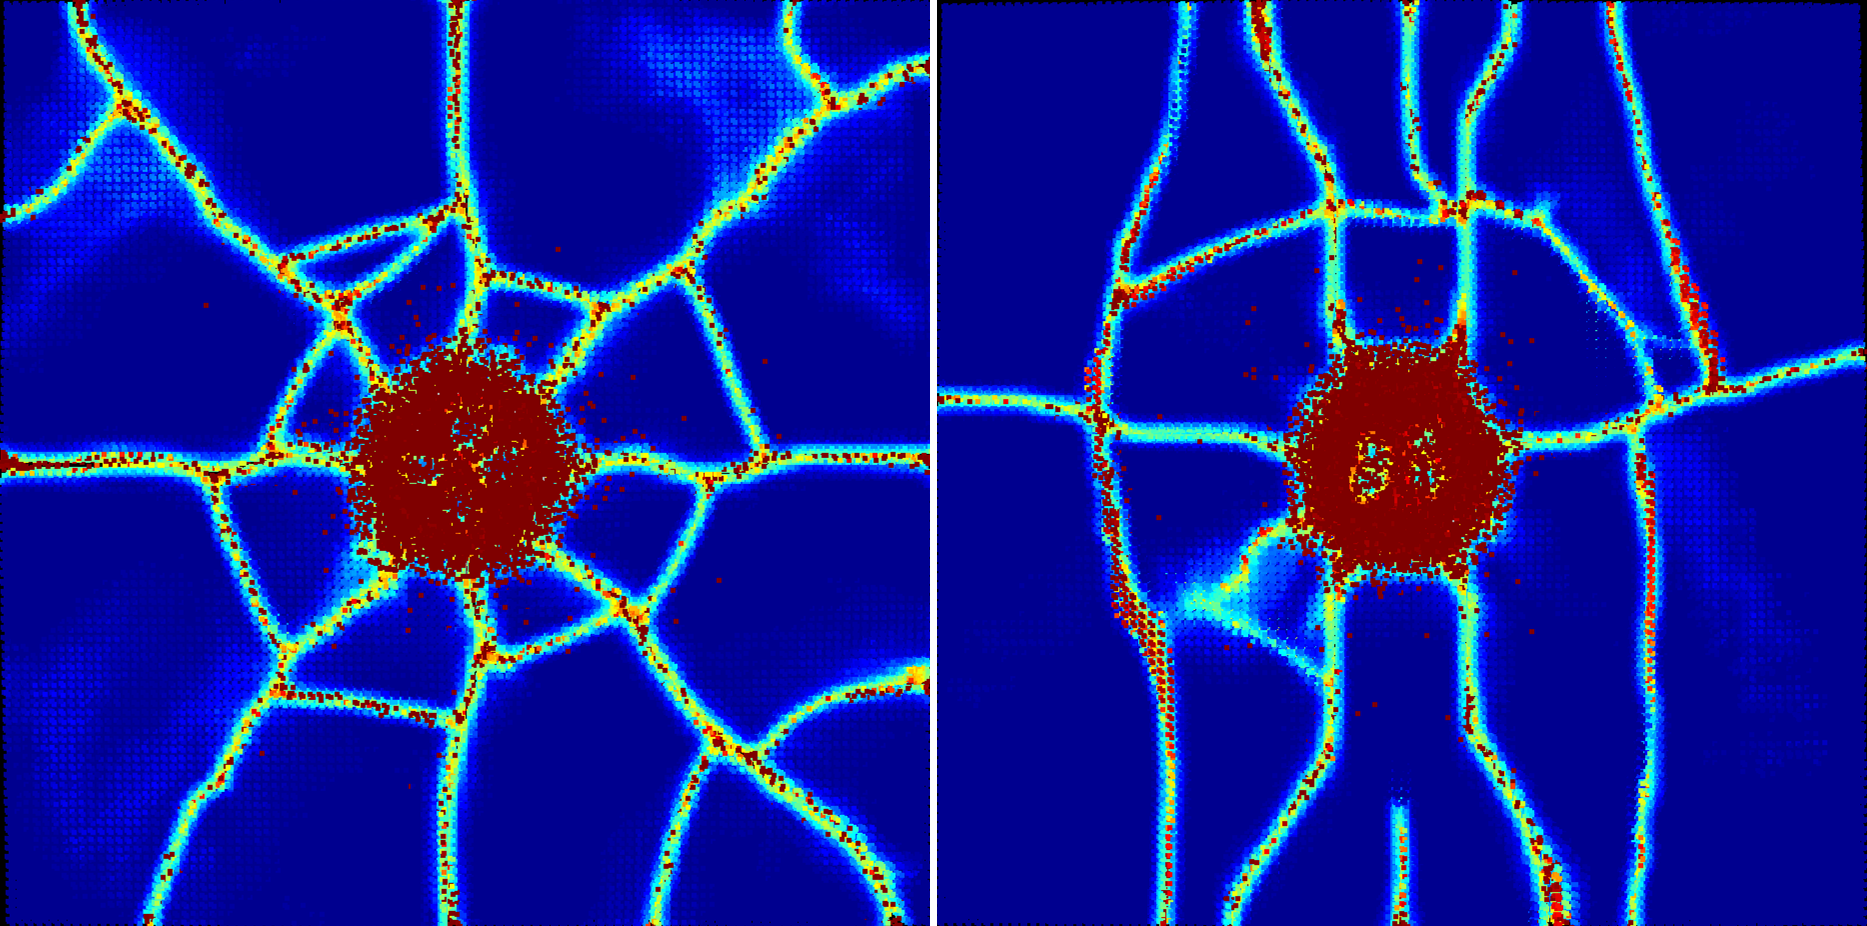
\includegraphics[width=0.6\linewidth]{chap/image/demo_impact_color_map}

  \caption{\label{demo_impact_color_map}
           各向同性碎裂(左图)和各向异性碎裂(右图)产生的碎裂模式对比。其中蓝色表示粒子未发生碎裂,而红色表示粒子已经完全发生碎裂。可以看到,在各向异性矩阵 $\mathbf{G}$ 的作用下,碎裂模式在 x,y 两个不同的方向明显不同,其中 x 方向更难发生碎裂,而 y 方向则相对更容易发生碎裂。
          }
\end{figure}

值得注意的是,事实上材质中的各向异性行为是极为复杂的,学术界也在提出不同的模型来进行解释。在本文工作中,我们仅仅是通过对权重函数来进行简单扩展,虽然取得了不错的各向异性碎裂效果,但在表达能力上仍然是有所欠缺的。现阶段关于近场动力学理论各向异性的更成熟模型仍有待探索。

\section{碎裂之拓扑更新}
在章节\label{discretization} 中,已经详细阐述了本文工作所采用的离散化框架,以及物体形变时通过加权平均的方式来对网格顶点的位置来进行更新。但对于碎裂问题,其改变的不仅仅是顶点的位置,而是同时需要改变其拓扑连接关系,因此这一问题相对于形变要更为复杂。

为方便讨论,我们将在二维情况下进行算法阐述,但将其拓展到三维是自然的,并不存在障碍。本文工作所提出的碎裂策略受\mycite{Chen}{2013}启发,同样是采用沿四面体边缘分割的方法,不过其仅仅针对脆性材料的碎裂仿真。沿四面体边界分离的策略还类似于工作\textcolor{blue}{(M\"{u}ller et al. 2001)\parencite{Muller2001}}。本文工作所用具体算法可如下图 \ref{topology_control} 所示。

\begin{figure}[!htb]
  \centering
  \captionsetup{justification=centering}
  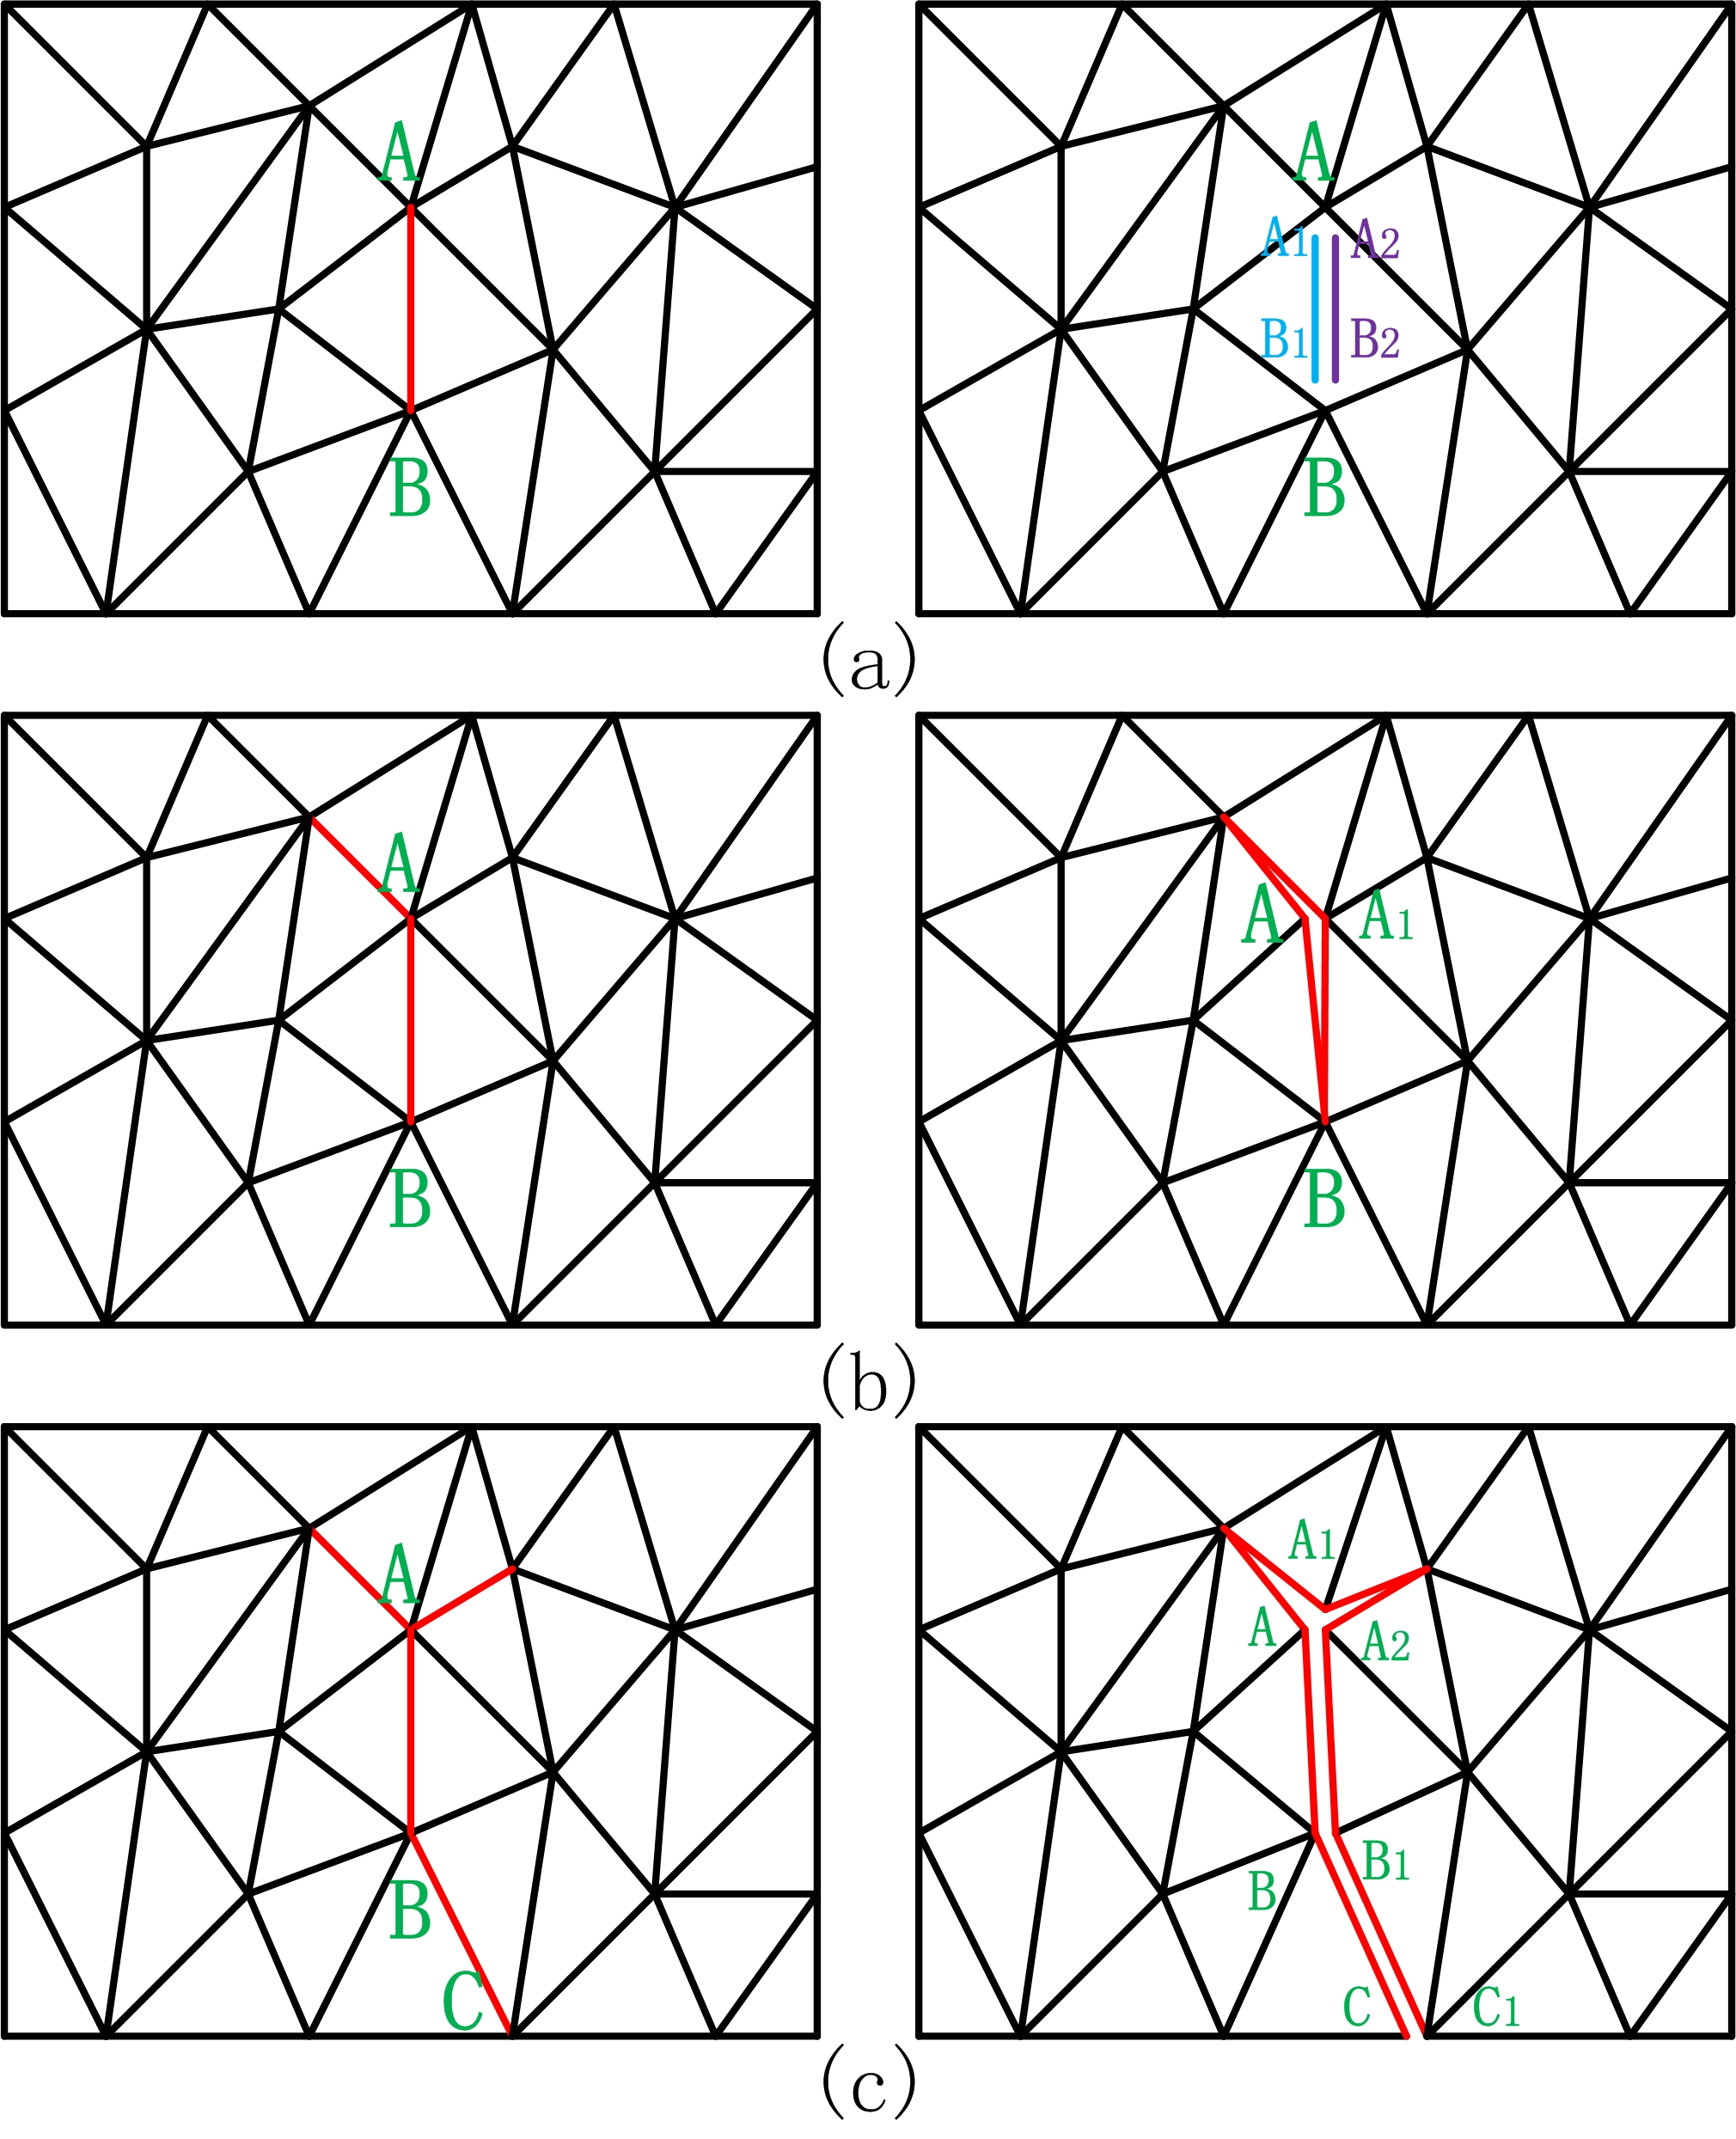
\includegraphics[width=0.6\linewidth]{chap/image/topology_control}
  \caption{\label{topology_control}
           碎裂之拓扑更新算法。图(a)表示在形变体发生碎裂时,单纯地复制碎裂边并不可取。图(b)表示将复制边策略转变为顶点分裂策略,当另一条碎裂边加入时,则可以将顶点进行分裂。图(c)表示多处同时发生碎裂。
          }
\end{figure}

如图\ref{topology_control}(a)中,当共享 AB 边的两个三角形(对应两个物理仿真粒子)发生碎裂时(三维情下对应共享面和四面体),对于脆性材料的碎裂,通常使用的策略是直接复制 AB 边,得到 $\texttt{A}_1\texttt{B}_1$ 和 $\texttt{A}_2\texttt{B}_2$。 但对于形变体的碎裂,这一策略并不可行,因为在脆性材料中可以认为这两条边是完全重合的,而在形变体中则不然,因此也无法决定使用$\texttt{A}_1$ 还是 $\texttt{A}_2$ 去替换原有顶点 A,以及使用 $\texttt{B}_1$ 还是 $\texttt{B}_2$ 去替换原有顶点 B。 为解决这一问题,我们将边复制(三维情况下对应面复制)问题转换为在 FEM 中常用的顶点分裂问题。如图\ref{topology_control} 所示,我们需要暂时推迟顶点 A 的分裂在拓扑上的反映,直到另外一条碎裂边(crack edge)加入。如此,我们便可以自然地将顶点 A 分裂成 $\texttt{A}_1$ 和 $\texttt{A}_2$,以反映碎裂引起的拓扑变化,因为此时这两条碎裂边已经将与顶点 A 相连的所有三角形隔离成不通过顶点 A 相连的两个独立部分。

在具体实现中,首先需要在仿真开始前遍历整个三角网格,并且为每个顶点存储其直接相连的三角形序号。在仿真过程中,我们仅仅需要考虑当前新产生碎裂边中所涉及的顶点,因为只有这些顶点才具有分裂的可能。对于每一个已经发生碎裂并可能需要进行分裂的顶点,我们判断与其相连的三角形是否已经被碎裂边隔离成不通过此顶点相连的两个独立部分。如果是此情形,则将顶点进行复制,并将其赋予给不同的三角形,即完成顶点的分裂过程。在顶点分裂之后,便可以将这些碎裂边进行删除,因为物体新的边界已经形成。如果与该顶点相连的三角形可以被分裂多个独立部分,则相应将顶点分裂成多份,如图\ref{topology_control}(c)所示。此外,如果同一碎裂边的多个顶点同时发生碎裂,此算法同样可以兼容。关于与顶点相连三角形的独立部分的具体查找,本文工作使用并查集 (disjoin set)算法来进行实现。

上述方法在理解上较为直观,实现上也并不复杂,并且能够取得非常逼真的视觉效果,具体详见\ref{fracture_results}章节。但值得注意的是,由于采用的是沿四面体边界分离的策略,而不是将四面体本身进行剖分,因此在碎裂过程中也容易产生不自然的锯齿形状。为缓解这一问题,本文工作的碎裂实验也往往在具有较高空间分辨率的四面体网格进行,以提供更多的几何细节。


\section{实验结果}
\label{fracture_results}
碎裂仿真实验运行环境和物体模型产生方法同形变仿真(章节\ref{deformation_results})一致。利用基于上述章节描述的碎裂模型和各向异性模型,本章节证明所提模型能够产生具有高逼真度的碎裂效果。

如图\ref{demo_impact}所示为不同材质的碎撞击裂实验,其中一个球以恒定速度分别穿过各向同性的脆性材料、各向异性的脆性材料、各向同性的塑性材料和各向异性的塑性材料,这一实验充分展示了本文所提方法所具备的能力,其能够对多种不同属性的材料进行仿真。我们相信本文工作为图形学领域第一次使用基于近场动力学理论的仿真框架来模拟如此多样化材质的碎裂现象。

\begin{figure}[!htb]
  \centering
  \captionsetup{justification=centering}
  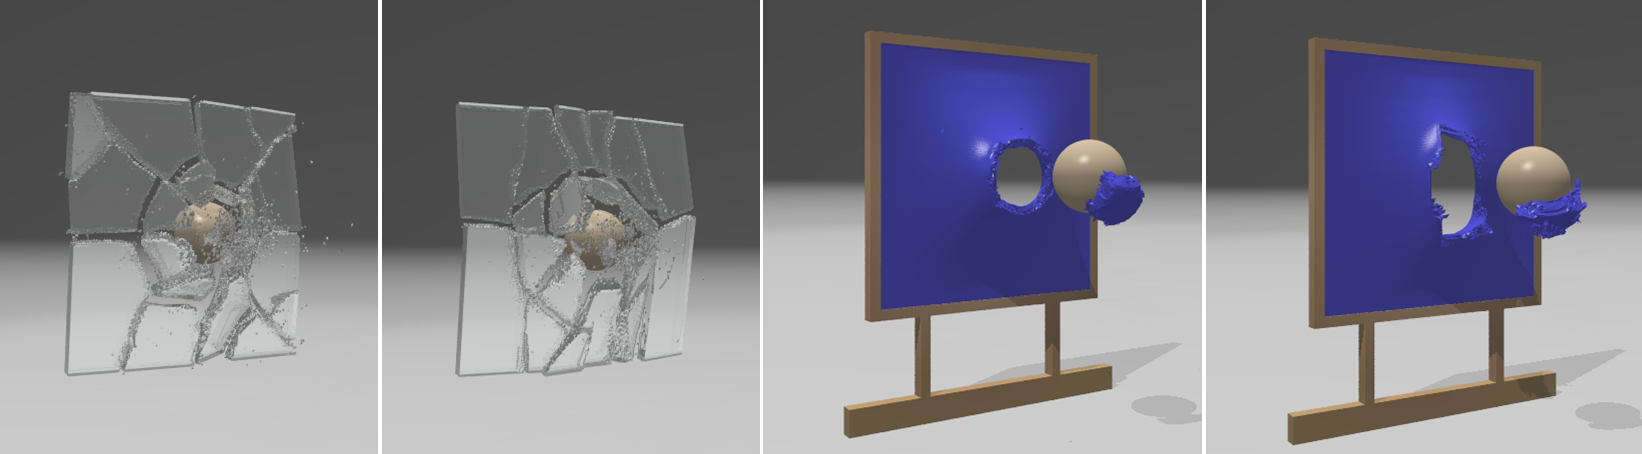
\includegraphics[width=\linewidth]{chap/image/demo_impact}

  \caption{\label{demo_impact}
           不同材质的撞击碎裂实验。球以恒定速度穿过不同材质构成的 Wall,产生不同的碎裂效果。从左到右分别为各向同性材质的脆性碎裂、各向异性材质的脆性碎裂、各向同性的塑性碎裂、各向异性的塑性碎裂。
          }
\end{figure}

图\ref{demo_impact_upside_plastic_fracture}表示具有具有不同塑性形变总量限制的可延展性碎裂实验。可以看到随着塑性总量的不同,物体的碎裂行为也有所改变。

\begin{figure}[!htb]
  \centering
  \captionsetup{justification=centering}
  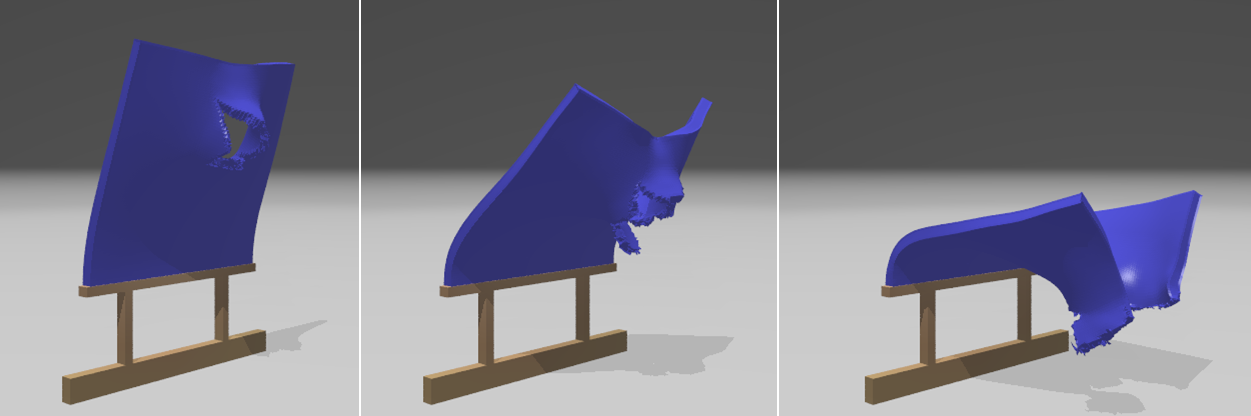
\includegraphics[width=\linewidth]{chap/image/demo_impact_upside_plastic_fracture}

  \caption{\label{demo_impact_upside_plastic_fracture}
           具有不同塑性形变总量限制的可延展性碎裂模拟,从左图到右图 $\frac{\gamma}{|\mathbf{x}_j-\mathbf{x}_i|}$ 分别为 0.1,0.15, 和 0.2.
          }
\end{figure}

图\ref{demo_tear_armadillo}展示了关于 Armadillo 的撕裂实验。仿真初始时,Armadillo 背部被固定,然后其四肢被以恒定速度撕扯,最终分离开来。这一实验充分显示本文所提方法能够仿真可延展性碎裂,以及多处同时发生的渐变式撕裂。图\ref{demo_tear_armadillo_close_view} 进一步展示了 Armadillo 撕裂实验的近视图。可以看到,当拉近摄像头时,还是可以较为明显地看出碎裂产生的锯齿状。因此,如果需要特别精细的碎裂效果,还需要更为高分辨率的物体模型,这也一定程度上说明本文方法在这一方面还存在缺陷,需要进一步改进。

\begin{figure}[!htb]
  \centering
  \captionsetup{justification=centering}
  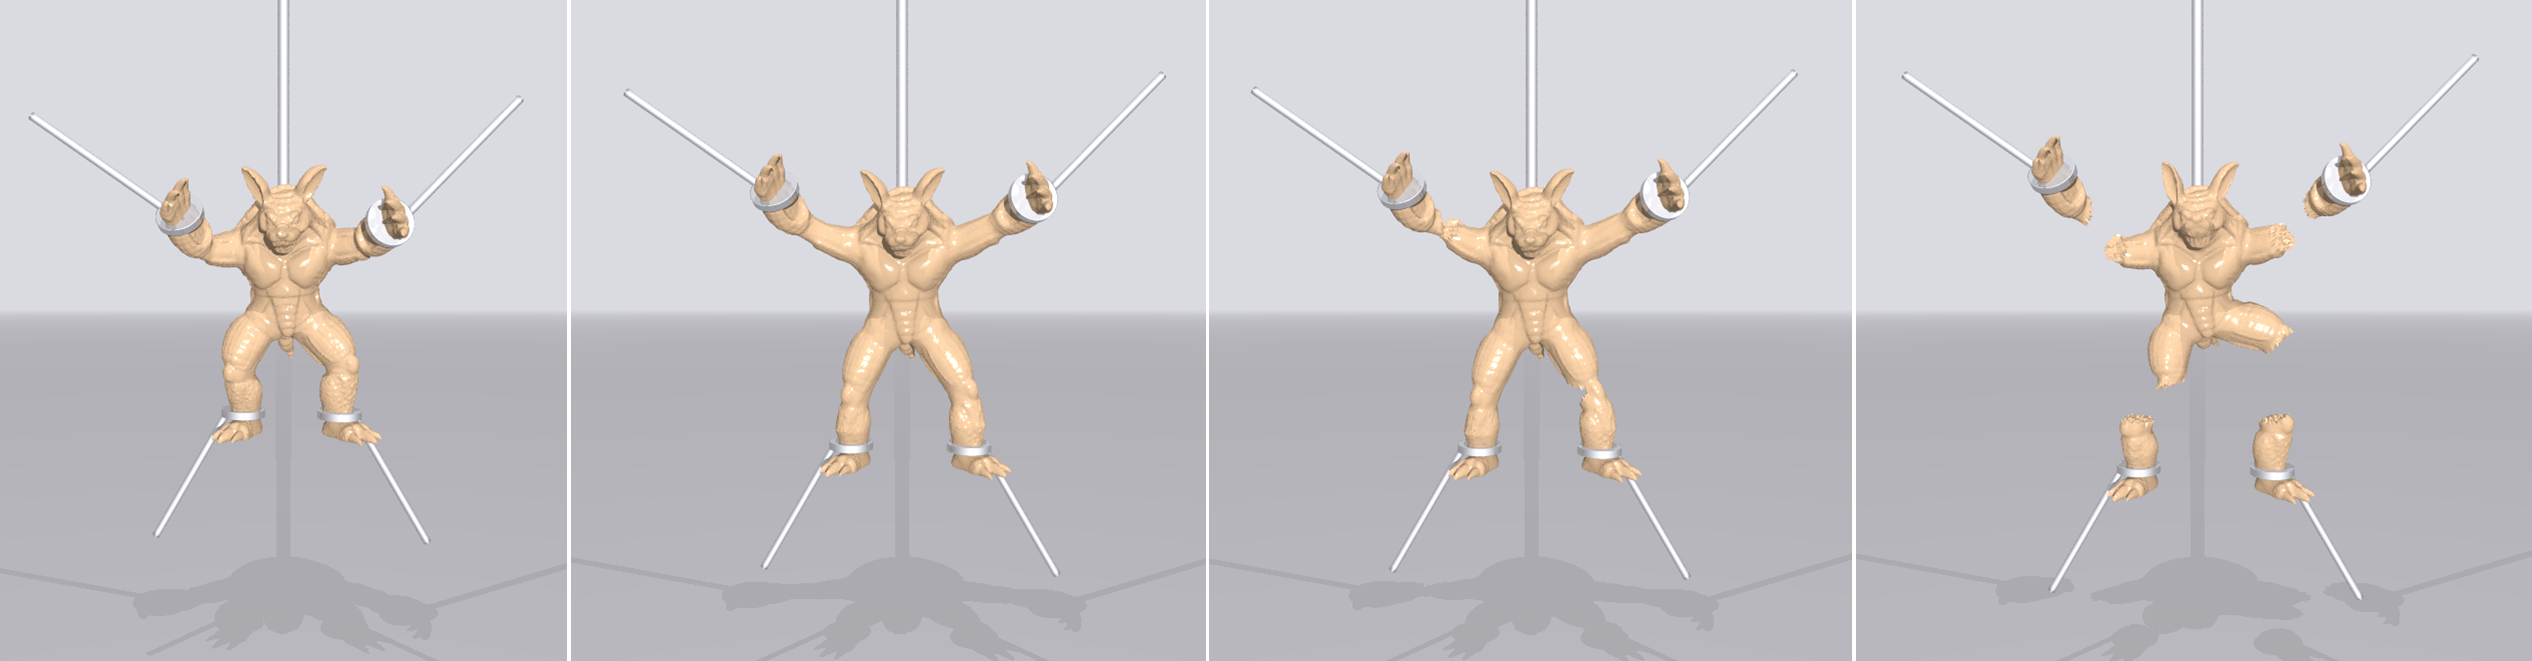
\includegraphics[width=\linewidth]{chap/image/demo_tear_armadillo}

  \caption{\label{demo_tear_armadillo}
           Armadillo 撕裂实验。Armadillo 其背部被固定,然后其四肢被撕扯裂开。
          }
\end{figure}

图\ref{demo_jello}所示为果冻穿透实验,一颗子弹以恒定速度穿过果冻,果冻被固定在地面,从而产生复杂的碎裂效果。

\begin{figure}[htbp]
\centering
\begin{minipage}[t]{0.45\textwidth}
\flushleft

  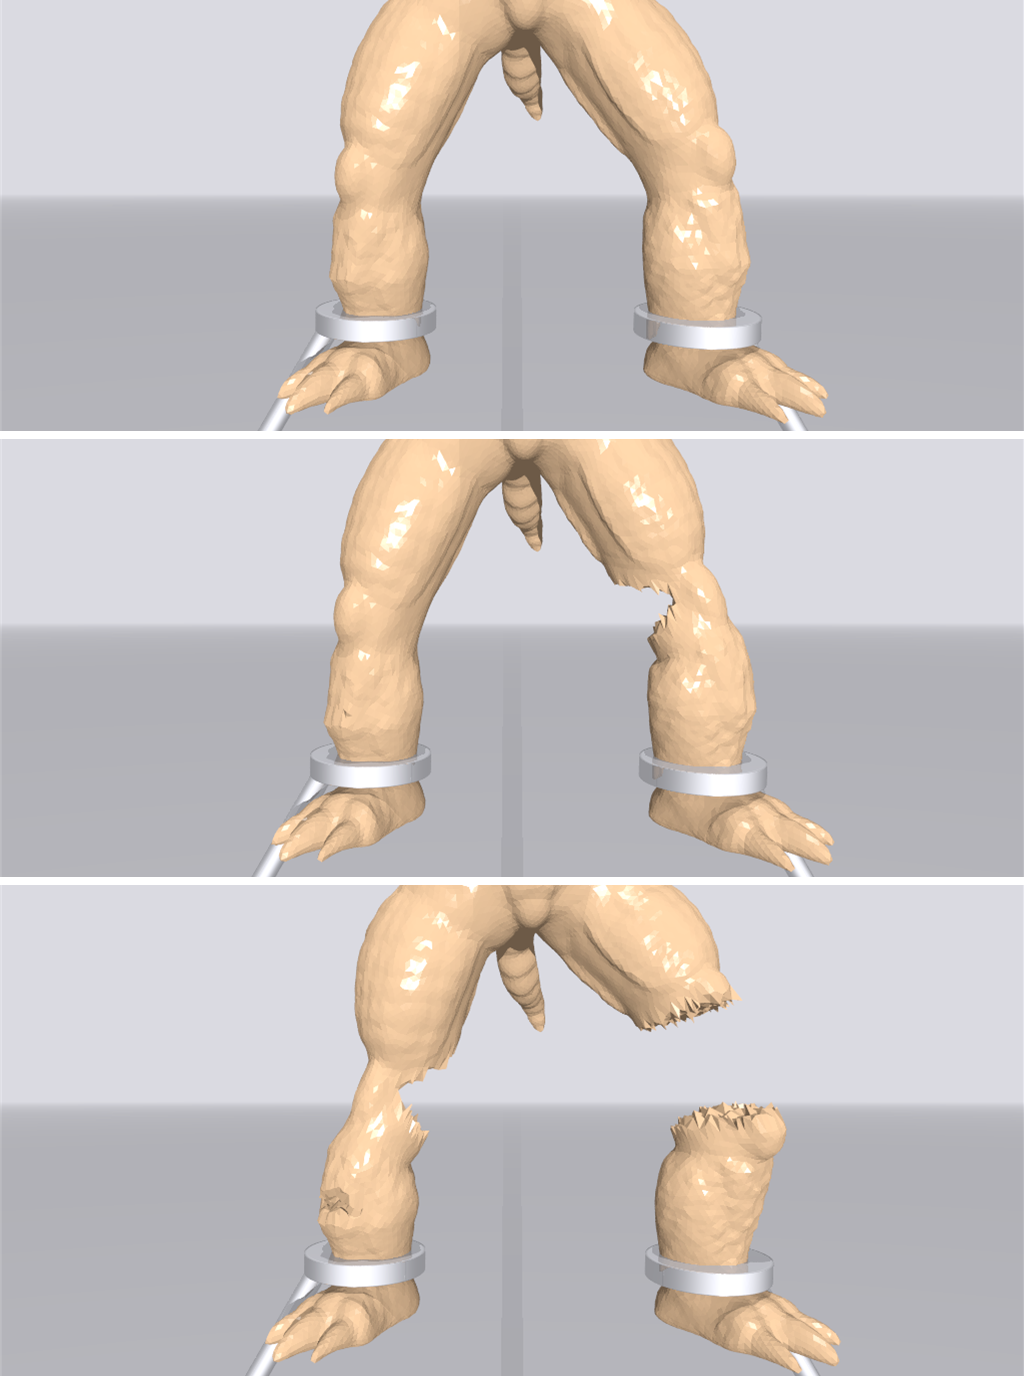
\includegraphics[width=0.9\linewidth]{chap/image/demo_tear_armadillo_close_view}
  \caption{\label{demo_tear_armadillo_close_view}
           Armadillo 撕裂实验近视图。\\从近处看,可以看到较为明显的\\锯齿状。
          }

\end{minipage}
\begin{minipage}[t]{0.45\textwidth}
\flushright

  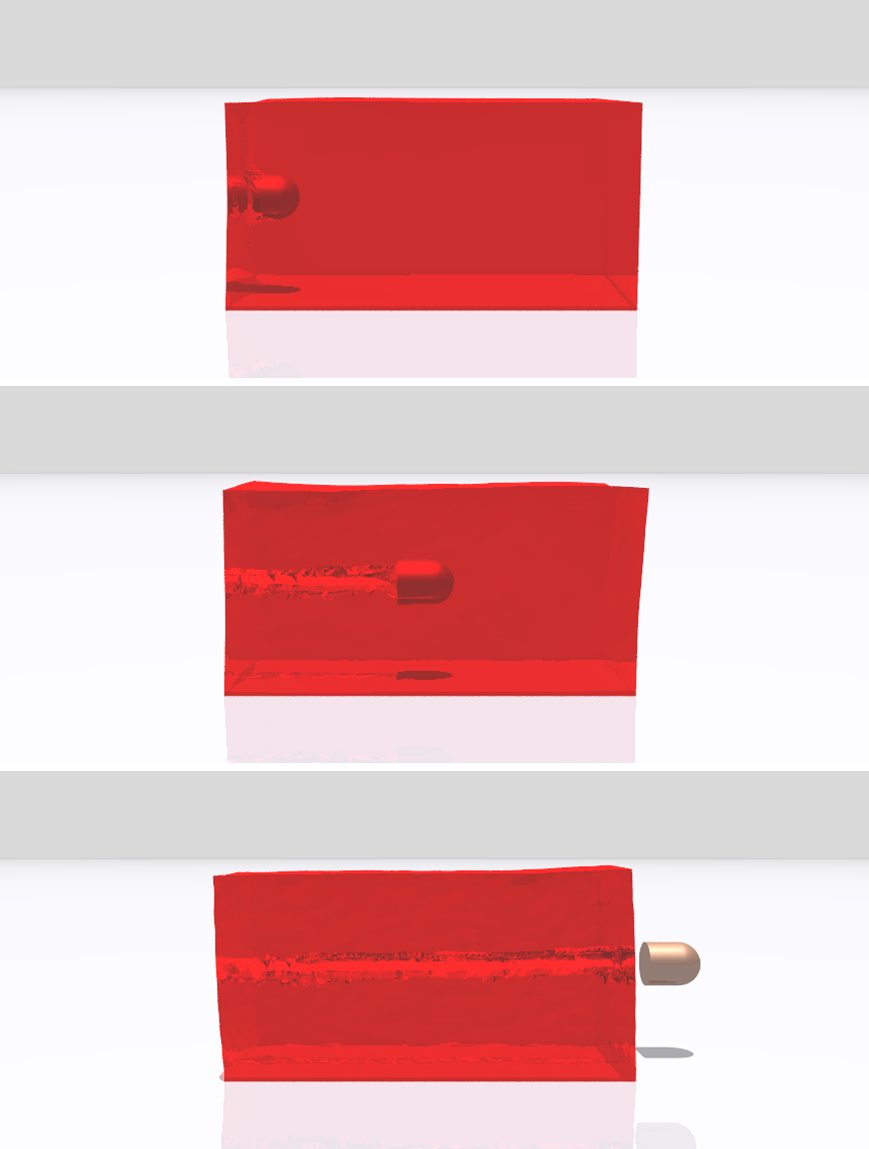
\includegraphics[width=0.9\linewidth]{chap/image/demo_jello}
  \caption{\label{demo_jello}
           果冻穿透实验。一颗子弹以恒定速度穿过果冻,产生碎裂效果。
          }

\end{minipage}
\end{figure}

图\ref{demo_brittle_fall}所示为球压玻璃板实验。玻璃板中心位置被放置一个金属球,并不断施加压力,使玻璃板发生碎裂。在这一例子中,可以清晰地看到裂纹的生长过程,效果非常惊艳。这一效果几乎不可能使用 level set 方法来实现\mycite{Hegemann}{2013},因为如此精细的裂纹需要极高空间分辨率的背景栅格。甚至对于传统 FEM 方法\textcolor{blue}{(O'Brien et al. 1999)\parencite{OBrien1999}},\textcolor{blue}{(O'Brien et al. 2002)\parencite{OBrien2002}}也是一个非常巨大的挑战,因为这一现象涉及到裂纹分支生长和合并的复杂碎裂行为,需要非常复杂 remeshing 操作。而利用本文方法,这一现象可以得到非常自然地处理。

\begin{figure}[!htb]
  \centering
  \captionsetup{justification=centering}
  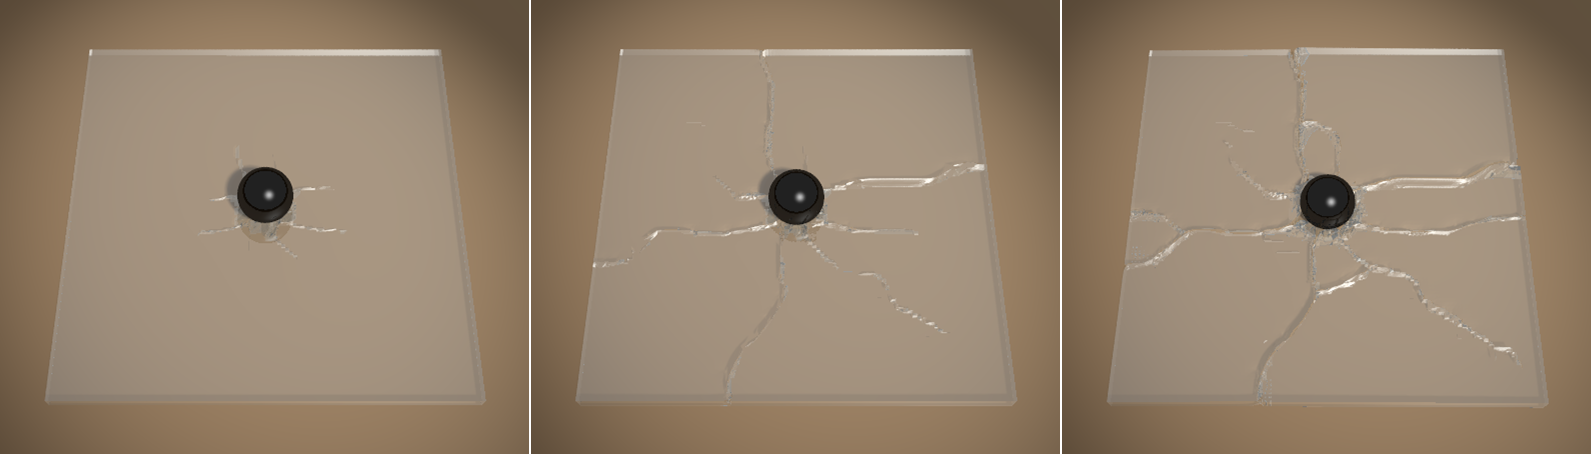
\includegraphics[width=\linewidth]{chap/image/demo_brittle_fall}

  \caption{\label{demo_brittle_fall}
           玻璃板受压实验。玻璃板中心位置被放置一个金属球,并不断施加压力,从而发生碎裂。图中可以看到明显裂纹生长过程,证明本文所提方法能够轻松处理裂纹分支的生长以及合并。
          }
\end{figure}

图\ref{demo_fall_bunny}所示为 Bunny 衰落实验。一个弹性 Bunny 摔落在地板上,并散成多块。从中可以看到本文方法的方法能够捕捉到材质的二次碎裂线性。

\begin{figure}[!htb]
  \centering
  \captionsetup{justification=centering}
  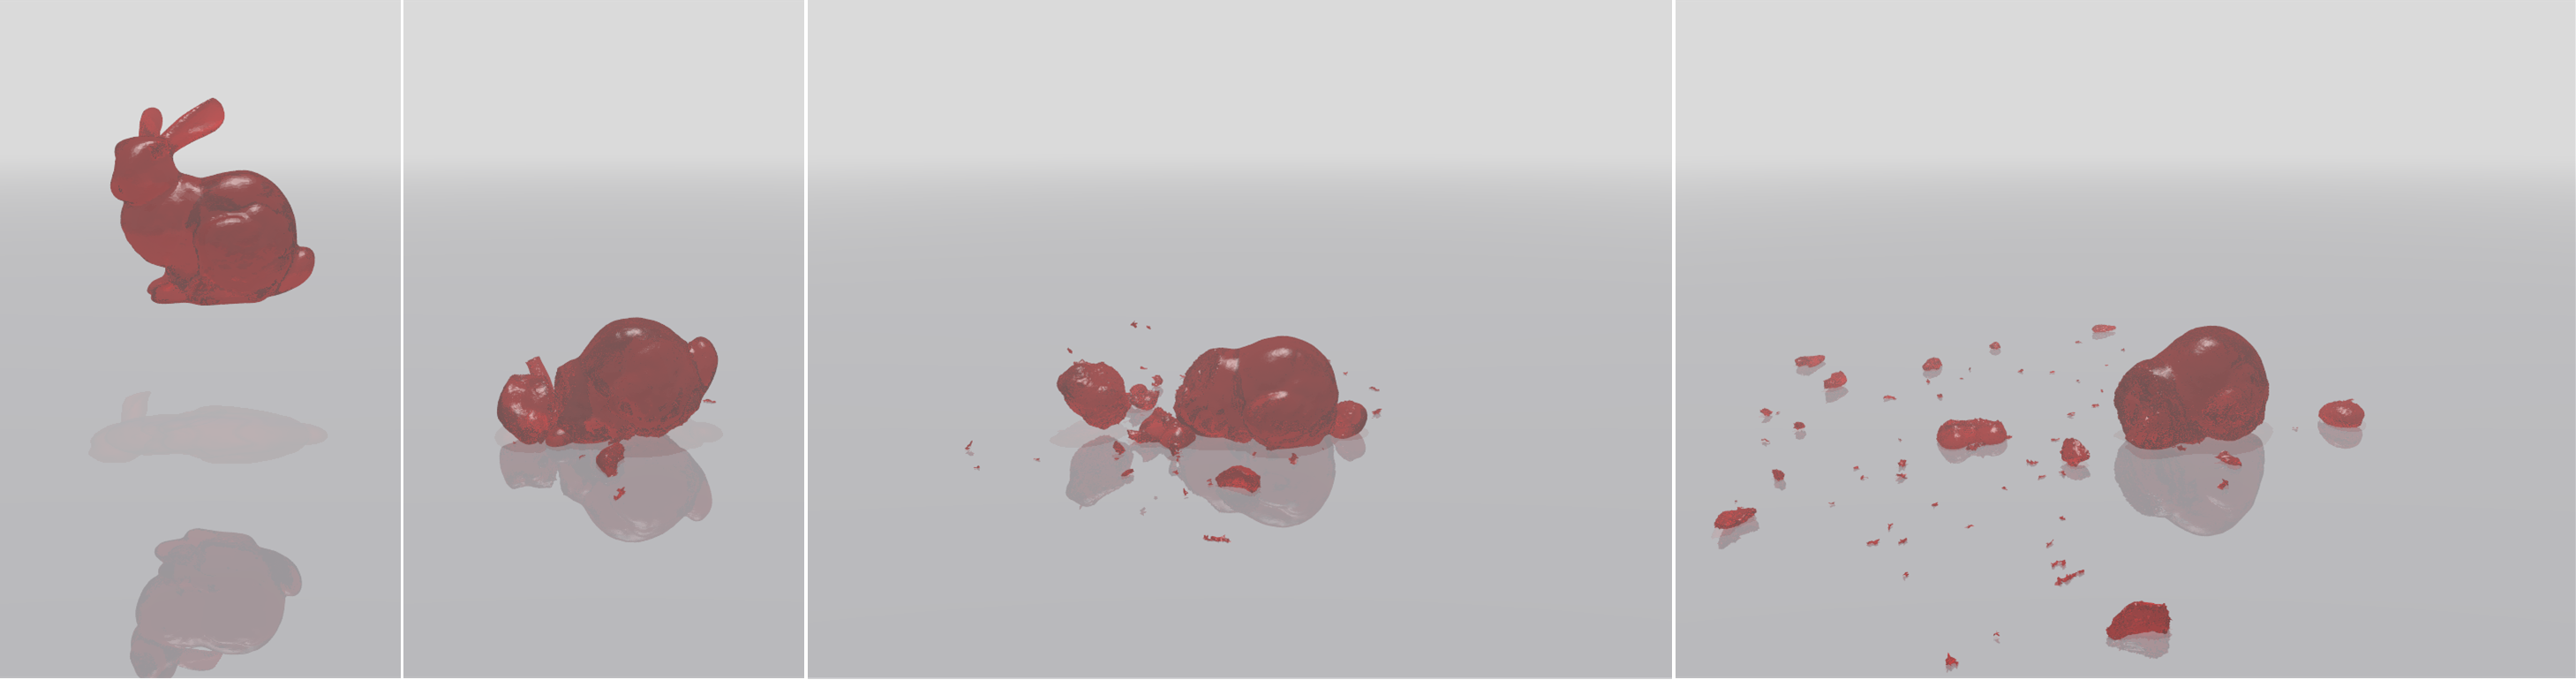
\includegraphics[width=\linewidth]{chap/image/demo_fall_bunny}

  \caption{\label{demo_fall_bunny}
           Bunny 摔落实验。一个弹性 Bunny 摔落在地板上,并散成多块。注意图中的二次碎裂效果。
          }
\end{figure}

最后一个实验为薄片撕裂实验,如图所示。在此实验中,弹性薄片从两边进行撕扯,最开始的开裂处位于边端,但裂纹随后扩展到整块薄片,将薄片分裂成多块。注意其中由于裂纹分支以及合并而产生的丝絮状细块(filaments)。

表\ref{fracture_results_table}展示了上述碎裂仿真实验所有模型参数以及物理参数。

\newpage
\begin{figure}[!htb]
  \centering
  \captionsetup{justification=centering}
  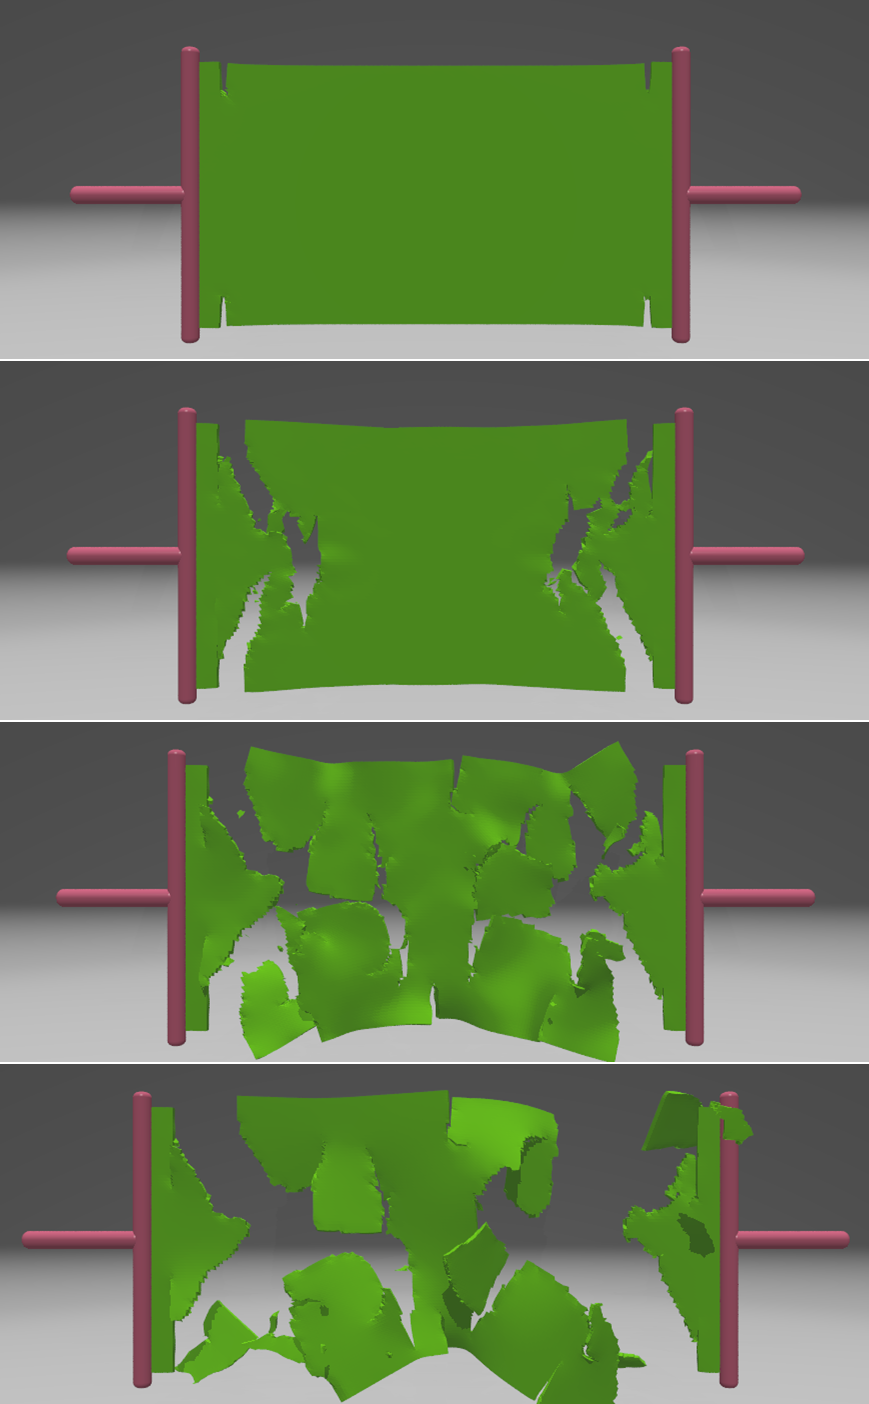
\includegraphics[width=0.6\linewidth]{chap/image/demo_tear_thin_sheet}

  \caption{\label{demo_tear_thin_sheet}
           薄片撕裂实验。薄片从两端开始撕裂,最终扩展到全部区域,注意其中的裂纹分支以及合并。
          }
\end{figure}

\begin{table*}[htb!]
\centerline{
\resizebox{1.3\textwidth}{!}{
\begin{tabular}{lccccccccccccc}
  \hline
  \hline
  Examples & particle num & $\delta$ & bond num & $\kappa$ & $\mu$ & $\rho$            & $\Psi_0$ & $\frac{\gamma}{|\mathbf{x}_j-\mathbf{x}_i|}$ & $s^w_{(k)(j)}$ & $\Delta t$ &$\lambda_a$    & $\lambda_l$  & performance\\
           &              &          &          &   (KPa)   & (KPa)  &(Kg/$\mathrm{m}^3)$&          &                                              &                & (s)       &   &   &(s/step)\\
  \hline
  Glass Wall[Figure~\ref{demo_impact}(a)(b),~\ref{demo_brittle_fall}]     & $3.0\times10^5$ & 1.45$\lambda$ & $5.0\times10^7$ & $3.3\times10^{7}$ & $2.0\times10^{7}$        & 2200 & $\infty $ & 0.0             & 0.0005   & $1.0\times10^{-6}$          &0&0& $\sim2.4$ \\
  Plastic Wall [Figure~\ref{demo_impact}(c)(d)]  & $3.0\times10^5$ & 1.45$\lambda$ & $5.0\times10^7$ & $3.3\times10^{3}$ & $2.0\times10^{3}$        & 2200 & $10^{25}$ & 0.2             & 0.05     & $1.0\times10^{-4}$          &$0.002$&0& $\sim2.4$ \\
  Wall [Figure~\ref{demo_impact_upside_plastic_fracture}]                & $3.0\times10^5$ & 1.45$\lambda$ & $5.0\times10^7$ & $1.0\times10^{4}$ & $6.0\times10^{3}$        & 1200 & $10^{26}$ &$(0.1,0.15,0.2)$ & 0.1  & $5.0\times10^{-5}$   &0.0005&0& $\sim2.4$ \\
  Jello [Figure~\ref{demo_jello}]               & $4.6\times10^5$ & 1.45$\lambda$ & $8.6\times10^7$ & $1.0\times10^3$   & $4.6\times10^2$          & 1000 & $\infty $ & 0.0             & 0.4      & $5.0\times10^{-5}$   &0&0& $\sim3.8$ \\
  Armadillo [Figure~\ref{demo_tear_armadillo}]          & $4.2\times10^5$ & 1.50$\lambda$ & $7.5\times10^7$ & $6.3\times10^4$   & $3.8\times10^4$          & 1000 & $\infty $ & 0.0             & 0.61     & $1.0\times10^{-4}$          &0&0.001& $\sim5.3$ \\
  Bunny [Figure~\ref{demo_fall_bunny}]              & $5.2\times10^5$ & 1.45$\lambda$ & $8.8\times10^7$ & $2.5\times10^2$   & $1.2\times10^2$          & 1000 & $\infty $ & 0.0             & 0.13     & $5.0\times10^{-4}$          &0&0& $\sim5.2$ \\
  Thin Sheet [Figure~\ref{demo_tear_thin_sheet}]              & $1.6\times10^5$ & 1.45$\lambda$ & $2.0\times10^7$ & $5.0\times10^3$   & $3.0\times10^3$          & 1000 & $\infty $ & 0.0             & 0.1     & $5.0\times10^{-5}$          &0&0.001& $\sim1.8$ \\
  \hline
\end{tabular}
}}
\caption{碎裂仿真中的模型参数、仿真参数、及效率数据。其中 $\lambda$ 是四面体网格的平均边长度,用于邻域的初始化。}
\label{fracture_results_table}
\end{table*}


\newpage
\section{本章小结}
本章主要研究基于近场动力学方法的弹塑性碎裂模拟。第一节给出了全文工作所用的碎裂模型,我们的模型主要基于 critical stretch,但对其进行了重要改进。本章第二节随即对原有的弹塑性本构模型作了重要的拓展,引入各向异性矩阵以支持各向异性碎裂现象的模拟。第三节则重点介绍了在章节\label{discretization}所述离散化框架的基础上,如何对拓扑结构进行更新,以在几何上反映材料的损伤,而基本思想是将面复制策略转变为顶点分裂策略。本章第四节则展示了本文方法所取得的效果。从实验结果来看,本文所提出模型能够较好地模拟弹塑性和各向异性材料的碎裂行为,并且能够很好地捕捉裂纹分支的生长以及合并现象。
